\documentclass{article}\usepackage[]{graphicx}\usepackage[]{color}
%% maxwidth is the original width if it is less than linewidth
%% otherwise use linewidth (to make sure the graphics do not exceed the margin)
\makeatletter
\def\maxwidth{ %
  \ifdim\Gin@nat@width>\linewidth
    \linewidth
  \else
    \Gin@nat@width
  \fi
}
\makeatother

\definecolor{fgcolor}{rgb}{0.345, 0.345, 0.345}
\newcommand{\hlnum}[1]{\textcolor[rgb]{0.686,0.059,0.569}{#1}}%
\newcommand{\hlstr}[1]{\textcolor[rgb]{0.192,0.494,0.8}{#1}}%
\newcommand{\hlcom}[1]{\textcolor[rgb]{0.678,0.584,0.686}{\textit{#1}}}%
\newcommand{\hlopt}[1]{\textcolor[rgb]{0,0,0}{#1}}%
\newcommand{\hlstd}[1]{\textcolor[rgb]{0.345,0.345,0.345}{#1}}%
\newcommand{\hlkwa}[1]{\textcolor[rgb]{0.161,0.373,0.58}{\textbf{#1}}}%
\newcommand{\hlkwb}[1]{\textcolor[rgb]{0.69,0.353,0.396}{#1}}%
\newcommand{\hlkwc}[1]{\textcolor[rgb]{0.333,0.667,0.333}{#1}}%
\newcommand{\hlkwd}[1]{\textcolor[rgb]{0.737,0.353,0.396}{\textbf{#1}}}%
\let\hlipl\hlkwb

\usepackage{framed}
\makeatletter
\newenvironment{kframe}{%
 \def\at@end@of@kframe{}%
 \ifinner\ifhmode%
  \def\at@end@of@kframe{\end{minipage}}%
  \begin{minipage}{\columnwidth}%
 \fi\fi%
 \def\FrameCommand##1{\hskip\@totalleftmargin \hskip-\fboxsep
 \colorbox{shadecolor}{##1}\hskip-\fboxsep
     % There is no \\@totalrightmargin, so:
     \hskip-\linewidth \hskip-\@totalleftmargin \hskip\columnwidth}%
 \MakeFramed {\advance\hsize-\width
   \@totalleftmargin\z@ \linewidth\hsize
   \@setminipage}}%
 {\par\unskip\endMakeFramed%
 \at@end@of@kframe}
\makeatother

\definecolor{shadecolor}{rgb}{.97, .97, .97}
\definecolor{messagecolor}{rgb}{0, 0, 0}
\definecolor{warningcolor}{rgb}{1, 0, 1}
\definecolor{errorcolor}{rgb}{1, 0, 0}
\newenvironment{knitrout}{}{} % an empty environment to be redefined in TeX

\usepackage{alltt}
\usepackage{graphicx}
\usepackage{float}
\usepackage{amsmath}
\usepackage{blindtext}
\usepackage[inline]{enumitem}
\usepackage{xcolor}
\usepackage{bm}
\usepackage {fancyvrb}
\usepackage {listings}
\usepackage[makeroom]{cancel}
\usepackage[urlcolor=blue,colorlinks=true]{hyperref}
\IfFileExists{upquote.sty}{\usepackage{upquote}}{}
\begin{document}

The beginning coordinates of the dihedral are:

\begin{align*}
  &S\ (0.138,0.0,-1.654)\\
  &C_1\ (0.474, 0.0, 1.059)\\
  &C_2\ (-0.621, 0.0, -0.007)\\
  &O\ (-0.125, 0.0, 2.357)
\end{align*}

When plotted this looks like this:

\begin{knitrout}
\definecolor{shadecolor}{rgb}{0.969, 0.969, 0.969}\color{fgcolor}
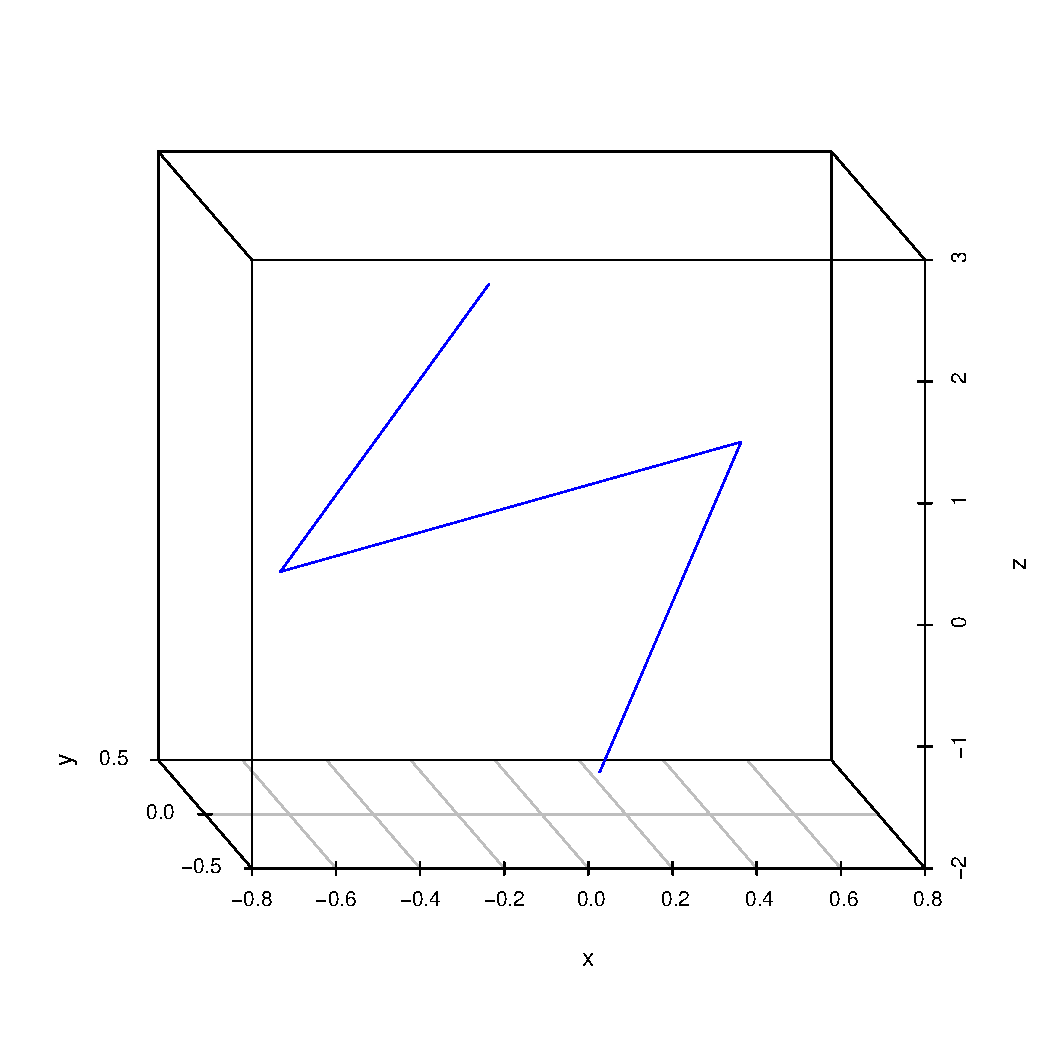
\includegraphics[width=\maxwidth]{figure/starting-dihedral-1} 

\end{knitrout}

We want to rotate the 4th atom $O$ about the dihedral axis which is defined by the $C-C$ vector.  This means the vector and the axis of rotation are:

\begin{align*}
  &\text{axis} = \vec{a} = \vec{C}_2-\vec{C}_1 = (-0.621-0.474,0.0-0.0,-0.007-1.059)=(-1.095,0.0,-1.066)\\
  &\text{vector} = \vec{v} = \vec{O}-\vec{C}_2 = (-1.25+0.621,0.0-0.0,2.357+0.007)=(-0.629,0.0,2.364)\\
  &\text{angle of rotation} = \theta = \frac{\pi}{2}
\end{align*}

The quaternion operator that defines this operation is (from \href{https://en.wikipedia.org/wiki/Quaternions_and_spatial_rotation}{Quaternions and Spatial Rotations - Wikipedia}):

\begin{align*}
  \vec{q} &= \cos(\frac{\pi}{4})+\sin(\frac{\pi}{4})\cdot \frac{1}{\| \vec{a} \|}\vec{a}\\
  \| \vec{a} \| &= \sqrt{(-1.095)^2+0^2+(-1.066)^2}=2.446\\
  \vec{q} &= \frac{1}{\sqrt{2}}+\frac{1}{2.446\sqrt{2}}(-0.629,0.0,2.364)=\frac{1}{\sqrt{2}}(1+(-0.257,\ 0.0,\ 0.966377))
\end{align*}

In addition we need the inverse which is obtained by just reversing the signs of the imaginary components:

$$\vec{q}^{\ -1}=\frac{1}{\sqrt{2}}(1+(0.257,\ -0.0,\ -0.966377)) $$

The rotated vector is then:
\begin{align*}
  \vec{v}_{new}&=\vec{q}(\vec{a})\vec{q}^{\ -1}\\
  \vec{q}(\vec{a})\vec{q}^{\ -1} &= (a_0+a_1\textbf{i}+a_2\textbf{j}+a_3\textbf{k})(0+v_1\textbf{i}+v_2\textbf{j}+v_3\textbf{k})(a_0-a_1\textbf{i}-a_2\textbf{j}-a_3\textbf{k})\\
  =&(a_0(v_1\textbf{i}+v_2\textbf{j}+v_3\textbf{k})+a_1(-v_1+v_2\textbf{k}-v_3\textbf{j})+a_2(-v_1\textbf{k}-v_2+v_3\textbf{i})+a_3(v_1\textbf{j}-v_2\textbf{i}-v_3))*\\
  &(a_0-a_1\textbf{i}-a_2\textbf{j}-a_3\textbf{k})\\
  =&((-a_1 v_1-a_2 v_2-a_3 v_3)+(a_0 v_1+a_2 v_3-a_3 v_2)\textbf{i}+(a_0 v_2-a_1 v_3+a_3 v_1)\textbf{j}+(a_0 v_3+a_1 v_2-a_2 v_1)\textbf{k})*\\
  &(a_0-a_1\textbf{i}-a_2\textbf{j}-a_3\textbf{k})\\
  &\text{Going term by term we get:}\\\\
  &(-a_1 v_1-a_2 v_2-a_3 v_3)=(-(-0.18173*-0.629)-(0.0*0.0)-(0.683332*2.364))=-1.7297\\
  &(a_0 v_1+a_2 v_3-a_3 v_2)\textbf{i}=(\frac{1}{\sqrt{2}}*(-0.629)+(0.0*2.364)-(0.68333*0.0))\textbf{i}=-0.445\textbf{i}\\
  &(a_0 v_2-a_1 v_3+a_3 v_1)\textbf{j}=(\frac{1}{\sqrt{2}}*0-(-0.18173*2.364)+(0.68333*-0.629))\textbf{j}=-0.00021\textbf{j}\\
  &(a_0 v_3+a_1 v_2-a_2 v_1)\textbf{k}=(\frac{1}{\sqrt{2}}*2.364+(-0.18173*0)-(0*-0.629))\textbf{k}=1.6716\textbf{k}\\\\
  &\text{Putting this back in the original equation we get:}\\\\
  &\vec{v}_{new} =(x_0+x_1\textbf{i}+x_2\textbf{j}+x_3\textbf{k})*(a_0-a_1\textbf{i}-a_2\textbf{j}-a_3\textbf{k})\\\\
  &\text{Applying the last multiplication we get:}\\\\
  &((x_0*a_0)-(x_1*-a_1)-(x_2*-a_2)-(x_3*-a_3))+\\
  &((x_0*-a_1)+(x_1*a_0)+(x_2*-a_3)-(x_3*-a_2))\textbf{i}+\\
  &((x_0*-a_2)-(x_1*-a_3)+(x_2*a_0)+(x_3*-a_1))\textbf{j}+\\
  &((x_0*-a_3)+(x_1*-a_2)-(x_2*-a_1)+(x_3*a_0))\textbf{k}
\end{align*}

\end{document}

















